\chapter{Bestimmung der Lage}
\label{chap:projektion}

Ein wichtiger Teil in der Augmented Reality ist die Lage (engl. pose) eines Objekts im dreidimensionalen Raum. Diese setzt sich aus der Position und der Rotation des Objekts in einem räumlichen Koordinatensystem zusammen. Oft werden diese auch \textit{extrinsische Parameter} genannt. Algorithmen zur Bestimmung dieser Parameter fallen in die Kategorie \textit{pose estimation}.
\\
\\
Im diesem Kapitel werden die verwendeten Methoden zur Lagebestimmung von Objekten erläutert.


\section{Lagebestimmung anhand des Schachbrettmusters}

% TODO: Bild Schachbrett

Um die Grundlagen der Lagebestimmung in der Augmented Reality zu verstehen und anzuwenden, macht es Sinn, die Grundfunktionalität anhand eines minimalen Beispiels zu entwickeln und dieses für das Hauptproblem dieser Thesis später zu erweitern. Dafür eignet sich besonders das bekannte Schachbrettmuster, da es in der Literatur und in Beispielen sehr oft verwendet wird, hauptsächlich zur Kalibration einer Kamera. Das Muster eignet sich gut, da es rechtechteckig ist, klare Kanten und Ecken aufweist und diverse Algorithmen zur Erkennung existieren, u.a. auch in OpenCV.

\subsection{Lösen des PnP Problems}

Wie bereits in Kapitel \ref{sec:projektionsmodell} angesprochen, wird in der Pose Estimation vom Pinhole-Kameramodell ausgegangen, in dem 3D Punkte im Raum auf eine Bildebene projiziert werden. Zur Bestimmung der Lage eines Objekts wird von der Gegenrichtung ausgegangen: Es wird versucht eine Menge von Punkten auf der zweidimensionalen Bildebene mittels einer kombinierten Rotations- und Translationsmatrix den korrespondierenden Objektpunkten zuzuordnen. Zur Lösung dieses Problems werden häufig sogenannte PnP Algorithmen eingesetzt. PnP wird in der Literatur als \textit{Perspective-n-Point-Problem} bezeichnet, wobei n für die Anzahl an Punktent steht. 

\paragraph{}
In OpenCV existieren diverse Funktionen, die gängige Algorithmen zur Positionsbestimmung implementieren. In diesem Projekt wird primär die Funktion \textit{solvePnP} eingesetzt.  Zur Ermittlung der benötigten Bildpunkte können für die erste Version der Positionsbestimmung ebenfalls auf OpenCV zurückgreifen, da die Erkennung eines beliebig grossen Schachbrettmusters  darin bereits implementiert wurde. 

\paragraph{}
Die $solvePnP$ Funktion in OpenCV unterstützt drei verschiedene Methoden zur Lösung eines PnP Problems:

\begin{itemize}

\item \textbf{Iterative Methode}
Diese Methode basiert auf der Levenberg-Marquardt Optimierung.

\item \textbf{P3P}
Basiert auf der Publikation von X.S. Gao, X.-R. Hou, J. Tang, H.-F. Chang ``Complete Solution Classification for the Perspective-Three-Point Problem''. Es werden exakt vier Objekt- und Bildpunkte benötigt.

\item \textbf{EPnP}
Diese Methode wurde durch F.Moreno-Noguer, V.Lepetit und P.Fua in der Publikation ``EPnP: Efficient Perspective-n-Point Camera Pose Estimation'' entwickelt.

\end{itemize}


\subsection{Definition der Objektpunkte}
\label{sec:definition-objektpunkte}

Ein wichtiger Schritt zur finalen Positionsbestimmung ist die Definition der Objektpunkte. Da wir bei einem Kamerabild keine Kenntnisse über die Dimensionen von Objekten haben, wird durch die definierten Objektpunkte ein eigenes Einheitensystem geschaffen. Da die Schachbretterkennung die Eckkanten zwischen den Flächen liefert, macht es Sinn für den Abstand der Objektpunkte den Wert 1 zu wählen. Somit beschreibt 1 Objekteinheit die Grösse eines Quadrates auf dem Schachbrett. Die Punkte werden grundsätzlich im dreidimensionalen Raum definiert, für den Fall des Schachbretts können wir jedoch z = 0 setzen, da alle Punkte sich in der selben Ebene befinden.

Weiter gilt es zu beachten, dass die definierten koordinaten der Objektpunkte einen Einfluss auf die resultierende Positionsmatrix haben. Der PnP Algorithmus berechnet die Position anhand des Ursprungs im Objektkoordinatensystem, d.h. die Matrix zeigt genau auf den Punkt (0, 0, 0). 
Da ein 3D Objekt auf die Mitte des Schachbretts projiziert werden soll, werden die Objektpunkte um diesen Nullpunkt konstriert, siehe Abbildung \ref{fig:object-points}.

\begin{figure}[!ht]
\centering
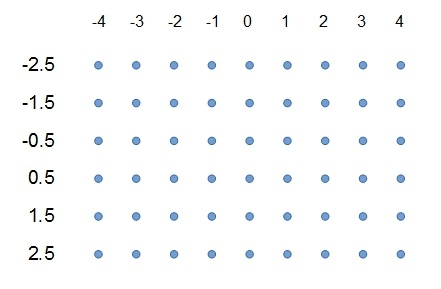
\includegraphics[scale=0.5]{images/object-points.jpg} 
\caption{Verteilung der Objektpunkt für ein Schachbrett.}
\label{fig:object-points}
\end{figure}


\subsection{Floating-point Ungenauigkeiten}

Ein Problem dass während des Projekts erst spät durch experimentieren gelöst werden konnte war, dass die berechnete und anschliessend dargestellte Projektion minimale Abweichungen aufweiste (siehe Abbildung \ref{floating-point-problem}). Das Problem war darauf zurückzuführen, dass die Algorithmen in OpenCV, die zur Lösung des PnP Problems verwendet wurden, scheinbar Probleme mit Gleitkommazahlen (engl. floating point) haben und dadurch das Resultat verfälschten.

Zur Lösung dieses Problems wurde ein möglichst einfacher Weg gewählt: Die Koordinaten der Objektpunkte wurden mit einem fix definierten Faktor von 100.0 hochskaliert. Dadurch wurden optisch erheblich bessere Resultate erzielt. Damit diese Methode anschliessend mit dem 3D-Rendering noch funktioniert, muss vor dem Rendering des 3D-Models die Model-View-Matrix entsprechend um den selben Skalierungsfaktor hochskaliert werden.

\begin{figure}[!ht]
\centering
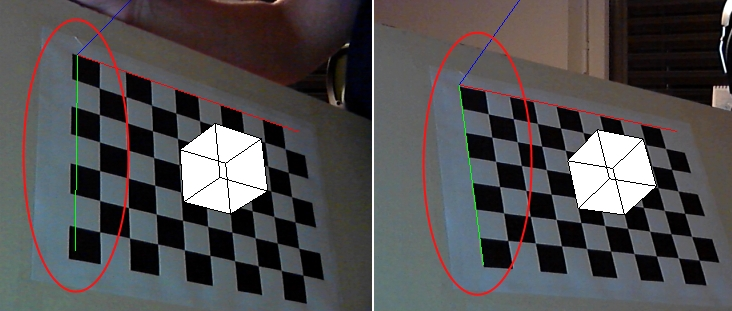
\includegraphics[scale=0.8]{images/floating-point-problem.jpg} 
\caption{Abweichung (links) vor der Optimierung (rechts).}
\label{fig:floating-point-problem}
\end{figure}


\section{Lagebestimmung einer Türe}

In diesem Kapitel wird die verwendete Methode zur Bestimmung der Lage einer Türe beschrieben.


\subsection{Grundidee}

\paragraph{}
Diese Grundidee zur Lagebestimmung einer Türe lässt sich anhand des Schachbrettmusters ableiten: Türe sowie Schachbrett sind beides rechteckige Objekte, dessen Eckpunkte ausserdem in der selben Ebene liegen. So wäre es physikalisch möglich, eine Türe mit dem Schachbrettmuster zu bemalen. 
Diese Idee wurde mit dieser Arbeit versucht virtuell zu entwickeln.
\\
\\
Als Input für die Lagebestimmung der Türe stehen genau deren vier Eckpunkte zur Verfügung. Diese werden von der Türerkennung generiert und bestehen aus einer X- und Y-Koordinaten, welche die Position eines Punktes im Ursprungsbild definieren. Ein erster Ansatz war, diese vier Bildpunkte weiteren vier vordefinierte Objektpunkten zuzuordnen und mittels eines PnP Algorithmus zu lösen. Die Objektpunkte wurden wie folgt definiert:

\begin{itemize}
\item \textbf{(0, 0)} oben links
\item \textbf{(1, 0)} oben rechts
\item \textbf{(1, 1)} unten rechts
\item \textbf{(0, 1)} unten links
\end{itemize}

Mit diesen Punkten wäre es theoretisch ebenfalls möglich, die Lage eines minimalen Schachbrettmusters (3x3) zu bestimmen. Das Problem im Falle einer Türe ist jedoch folgendes: Bei einem Schachbrettmuster sind die schwarzen bzw. weissen Flächen \textit{immer} Quadrate. Aus diesem Grund können die Objektpunkte ebenfalls als Quadrat definiert werden. Falls jedoch mit diesen Objektpunkten versucht wird die Lage eines nicht quadratischen Objekts, z.B. eine Türe, zu bestimmen, erhält man falsche Resultate. Da eine Türe auch kein standardisiertes Grössenverhältnis hat kann man keine vordefinierten Objektpunkte zur Lösung des Problems verwenden.

\subsection{Bestimmung des Grössenverhältnisses}

% TODO: evtl. noch Formeln aus Paper herleiten

\paragraph{}
In einer Arbeit von Zhengyou Zhang \cite{zhangrectification} wurde ein Verfahren entwickelt, mit welchem anhand genau vier Punkten eines Rechtecks dessen Grössenverhältnis berechnet werden kann. Hintergrund dieser Arbeit ist das automatische Erkennen von perspektivisch aufgenommenen Whiteboards mit anschliessender perspektivischen Entzerrung des Whiteboard-Inhalts.

Die Theorie funktioniert, weil bei den gegebenen Eckpunkten davon ausgegangen wird, dass diese sich in der gleichen Ebene befinden, was natürlich bei einem Whiteboard zutrifft. Aus diesem Grund kann auch für die Bestimmung des Grössenverthältnisses einer Türe dieses Verfahren herangezogen werden.

In Zhangs Dokument wird grundsätzlich von einer unkalibrierten Kamera ausgegangen und setzt bestimmte Kameraeigenschaften voraus, z.B. dass der Bildmittelpunkt genau in der Mitte ist, was bei einer Kamera nicht unbedingt der Fall sein muss. Zhang erwähnt auch, dass die Verzerrung der Kamera die Fehlerrate erhöhen kann. Da wir in unserem Modell von einer kalibrierten Kamera ausgehen, sind uns intrinsische Parameter und Verzerrung bekannt. Wir können deshalb vor der Anwendung des Algorithmus die Bildpunkte vorher entzerren.


\subsection{Messungen Grössenverhältnisse}

\paragraph{}
Zur Verifizierung der vorangehenden Arbeit von Zhang \cite{zhangrectification} wurden mit einer Spiegelreflexkamera hochauflösende Bilder einer Türe aufgenommen. Die Bilder wurden mit einem fixen Abstand zur Türe aufgenommen und ausgehend von der Türwand mit den Winkeln $10^\circ$, $30^\circ$, $50^\circ$, $70^\circ$ und $90^\circ$ aufgenommen. Anschliessend wurden die Koordinaten der vier Eckpunkte der Türe von Hand ausgelesen und mittels Algorithmus das Grössenverhältnis berechnet. Dieses wurde mit dem berechneten Verhältnis von \textbf{2.07} der aufgenommenen Türe mit den Massen \textbf{98.50cm x 204.00cm} verglichen.

\begin{center}
	\resizebox{\linewidth}{!}{%
    \begin{tabular}{ || l || l | l | l || l | l | l ||}
    \hline
    Winkel [$^\circ$] & Verhältnis (verzerrt) & Abweichung & Fehler & Verhältnis (entzerrt) & Abweichung & Fehler \\ \hline
    90 & 2.02 & 0.05 & 2.4 & 2.01 & 0.06 & 3.1 \\ \hline
    70 & 2.06 & 0.01 & 0.4 & 1.96 & 0.11 & 5.3 \\ \hline
    50 & 2.02 & 0.05 & 2.2 & 1.89 & 0.18 & 8.8 \\ \hline
    30 & 1.97 & 0.10 & 4.8 & 1.83 & 0.25 & 11.8 \\ \hline
    10 & 1.90 & 0.17 & 8.1 & 1.79 & 0.28 & 13.4 \\ \hline
    \end{tabular}
    }
\end{center}


\begin{figure}[!ht]
  \centering
  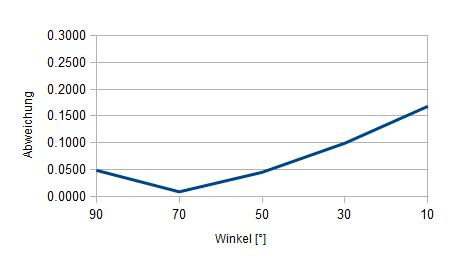
\includegraphics[width=0.75\linewidth]{images/ratio_v1_dist.jpg}
  \caption{Abweichung Grössenverhältnisse ohne Entzerrung, 1. Kalibration}
  \label{fig:ratio-v1-dist}
\end{figure}

\begin{figure}[!ht]
  \centering
  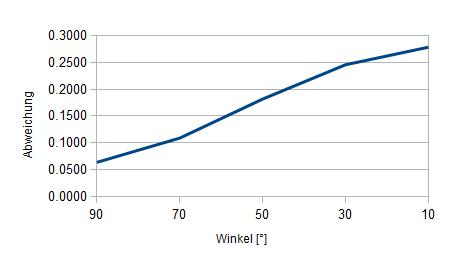
\includegraphics[width=0.75\linewidth]{images/ratio_v1_undist.jpg}
  \caption{Abweichung Grössenverhältnisse mit Entzerrung, 1. Kalibration}
  \label{fig:ratio-v1-undist}
\end{figure}


Die erste Durchführung der Messungen ergab ein unerwartetes Ergebnis. Der Verhältnis-Algorithmus wurde sowohl auf die verzerrten als auch die entzerrten Punkten angewendet. Überraschenderweise erhielten wir in der entzerrten Version schlechtere Resultate, was bei einer Spiegelreflexkamera verwunderlich ist, da diese eine sehr geringe Verzerrung haben sollte bzw. eine Entzerrung kameraseitig bereits durchführen sollte (siehe Abbildungen \ref{fig:ratio-v1-dist} und \ref{fig:ratio-v1-undist}).
\\
\\
Der Versuch wurde also ein zweites Mal gemacht. Diesmal wurde das Schachbrett zur Kalibration auf einer Spanpressblatte angebracht und möglichst flach aufgeklebt.


\begin{center}
	\resizebox{\linewidth}{!}{%
    \begin{tabular}{ || l || l | l | l || l | l | l ||}
    \hline
    Winkel [$^\circ$] & Verhältnis (verzerrt) & Abweichung & Fehler & Verhältnis (entzerrt) & Abweichung & Fehler \\ \hline
    90 & 2.01 & 0.06 & 2.7 & 2.01 & 0.06 & 2.8 \\ \hline
    70 & 2.03 & 0.04 & 2.0 & 2.03 & 0.03 & 1.8 \\ \hline
    50 & 2.03 & 0.04 & 1.8 & 2.04 & 0.03 & 1.4 \\ \hline
    30 & 2.06 & 0.01 & 0.3 & 2.06 & 0.01 & 0.3 \\ \hline
    10 & 2.07 & 0.00 & 0.0 & 2.06 & 0.01 & 0.7 \\ \hline
    \end{tabular}
    }
\end{center}

\begin{figure}[!ht]
  \centering
  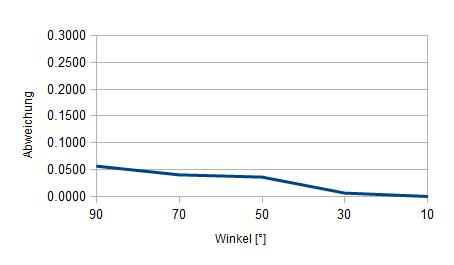
\includegraphics[width=0.75\linewidth]{images/ratio_v2_dist.jpg}
  \caption{Abweichung Grössenverhältnisse ohne Entzerrung, 2. Kalibration}
  \label{fig:ratio-v2-dist}
\end{figure}

\begin{figure}[!ht]
  \centering
  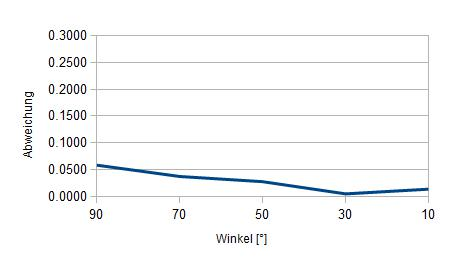
\includegraphics[width=0.75\linewidth]{images/ratio_v2_undist.jpg}
  \caption{Abweichung Grössenverhältnisse mit Entzerrung, 2. Kalibration}
  \label{fig:ratio-v2-undist}
\end{figure}


Die zweiten Resultate entsprachen nun den erwarteten Werten. Auf den Abbildungen \ref{fig:ratio-v2-dist} und \ref{fig:ratio-v2-undist}) ist gut zu erkennen, dass sowohl die verzerrte als auch die entzerrte Version ähnliche Resultate zurückliefert, was von einer Spiegelreflexkamera erwartet werden sollte. Zudem haben wir einen maximalen Fehlerwert von 2.8 Prozent messen können, was ein guter Wert ist. Der Versuch hat zudem gezeit, dass eine schlecht kalibrierte Kamera erhebliche Verfälschungen des Resultats zur Folge haben kann. 


\subsection{Umsetzung}
\label{sec:projektion-door}

\paragraph{}
Da nun, wie in den vorherigen Abschnitten beschrieben, das Grössenverhältnis der Türe berechnet werden kann, können wir den ursprünglichen Ansatz mit dem zuordnen von Objektpunkten weiterverfolgen. Die Objektpunkte werden nun jedoch nicht vordefiniert, sondern bei der Lagebestimmung automatisch anhand des Grössenverhältnisses generiert. Dabei wird als \textbf{Breite 1} angenommen und als \textbf{Höhe das Verhältnis r}. Die generierten Punkte werden wie folgt generiert:

\begin{itemize}
\item \textbf{(0, 0)} unten links
\item \textbf{(0, r)} oben links
\item \textbf{(1, r)} oben rechts
\item \textbf{(0, 1)} unten rechts
\end{itemize}

Diese Punkte können nun zusammen mit den erkannten Eckpunkten der Türe an einen PnP Algorithmus übergeben werden, welcher die Position und Rotation berechnet.

